% --- LaTeX Lecture Notes Template - S. Venkatraman ---

% --- Set document class and font size ---

\documentclass[letterpaper, 12pt]{article}


% --- Package imports ---

% Extended set of colors
\usepackage[dvipsnames]{xcolor}

\usepackage{
  amsmath, amsthm, amssymb, mathtools, dsfont, units,          % Math typesetting
  graphicx, wrapfig, subfig, float,                            % Figures and graphics formatting
  listings, color, inconsolata, pythonhighlight,               % Code formatting
  fancyhdr, sectsty, hyperref, enumerate, enumitem, framed }   % Headers/footers, section fonts, links, lists

% lipsum is just for generating placeholder text and can be removed
\usepackage{hyperref, lipsum} 
% \usepackage{bm}
% \usepackage{subfig}

% --- Fonts ---

\usepackage{newpxtext, newpxmath, inconsolata}
\usepackage{amsfonts}
\usepackage{pgfplots}
\pgfplotsset{compat=1.12}
\usepackage{tkz-fct}
\usepackage{svg}
\usepackage{tikz}
\usepackage{tikz-cd}
\usepackage{lipsum}
\usepackage{enumitem}
\usepackage[title]{appendix}
% \usepackage[toc,page]{appxendix}
\usepackage[utf8]{inputenc}
\usepackage{multicol}
\usepackage{multirow}
\usepackage{booktabs}

\usepackage{minted}  % code highlighting
% \usepackage[finalizecache,cachedir=.]{minted}
% \usepackage[frozencache,cachedir=.]{minted}

\DeclareUnicodeCharacter{3BC}{$\pi$}
\DeclareUnicodeCharacter{3C0}{$\pi$}

\usepackage[most]{tcolorbox}
\newtcolorbox{myquote}[1][]{%
  colback=black!5,
  colframe=black!5,
  notitle,
  sharp corners,
  % borderline west={2pt}{0pt}{red!80!black},
  enhanced,
  breakable,
}

\renewcommand*\pod[1]{%
  \allowbreak
  \mathchoice
    {\mkern 18mu}%
    {\mkern  8mu}%
    {\mkern  6mu}% "6mu" matches the space *after* the word "mod"
    {\mkern  6mu}%
  (#1)%
}

% --- Page layout settings ---

% Set page margins
\usepackage[left=1.35in, right=1.35in, top=1.0in, bottom=.9in, headsep=.2in, footskip=0.35in]{geometry}

% Anchor footnotes to the bottom of the page
\usepackage[bottom]{footmisc}

% Set line spacing
\renewcommand{\baselinestretch}{1.2}

% Set spacing between paragraphs
\setlength{\parskip}{1.3mm}

% Allow multi-line equations to break onto the next page
\allowdisplaybreaks

% --- Page formatting settings ---

% Set image captions to be italicized
\usepackage[font={it,footnotesize}]{caption}

% Set link colors for labeled items (blue), citations (red), URLs (orange)
\hypersetup{colorlinks=true, linkcolor=RoyalBlue, citecolor=RedOrange, urlcolor=ForestGreen}

% Set font size for section titles (\large) and subtitles (\normalsize) 
\usepackage{titlesec}
% \titleformat{\section}{\large\bfseries}{{\fontsize{19}{19}\selectfont\textreferencemark}\;\; }{0em}{}
\titleformat{\section}{\large\bfseries}{\thesection\;\;\;}{0em}{}
\titleformat{\subsection}{\normalsize\bfseries\selectfont}{\thesubsection\;\;\;}{0em}{}

% Enumerated/bulleted lists: make numbers/bullets flush left
%\setlist[enumerate]{wide=2pt, leftmargin=16pt, labelwidth=0pt}
\setlist[itemize]{wide=0pt, leftmargin=16pt, labelwidth=10pt, align=left}

% --- Table of contents settings ---

\usepackage[subfigure]{tocloft}

% Reduce spacing between sections in table of contents
\setlength{\cftbeforesecskip}{.9ex}

% Remove indentation for sections
\cftsetindents{section}{0em}{0em}

% Set font size (\large) for table of contents title
\renewcommand{\cfttoctitlefont}{\large\bfseries}

% Remove numbers/bullets from section titles in table of contents
\makeatletter
\renewcommand{\cftsecpresnum}{\begin{lrbox}{\@tempboxa}}
\renewcommand{\cftsecaftersnum}{\end{lrbox}}
\makeatother

% --- Set path for images ---

\graphicspath{{Images/}{../Images/}}

% --- Math/Statistics commands ---

% Add a reference number to a single line of a multi-line equation
% Usage: "\numberthis\label{labelNameHere}" in an align or gather environment
\newcommand\numberthis{\addtocounter{equation}{1}\tag{\theequation}}

% Shortcut for bold text in math mode, e.g. $\b{X}$
\let\b\mathbf

% Shortcut for bold Greek letters, e.g. $\bg{\beta}$
\let\bg\boldsymbol

% Shortcut for calligraphic script, e.g. %\mc{M}$
\let\mc\mathcal

% \mathscr{(letter here)} is sometimes used to denote vector spaces
\usepackage[mathscr]{euscript}

% Convergence: right arrow with optional text on top
% E.g. $\converge[p]$ for converges in probability
\newcommand{\converge}[1][]{\xrightarrow{#1}}

% Weak convergence: harpoon symbol with optional text on top
% E.g. $\wconverge[n\to\infty]$
\newcommand{\wconverge}[1][]{\stackrel{#1}{\rightharpoonup}}

% Equality: equals sign with optional text on top
% E.g. $X \equals[d] Y$ for equality in distribution
\newcommand{\equals}[1][]{\stackrel{\smash{#1}}{=}}

% Normal distribution: arguments are the mean and variance
% E.g. $\normal{\mu}{\sigma}$
\newcommand{\normal}[2]{\mathcal{N}\left(#1,#2\right)}

% Uniform distribution: arguments are the left and right endpoints
% E.g. $\unif{0}{1}$
\newcommand{\unif}[2]{\text{Uniform}(#1,#2)}

% Independent and identically distributed random variables
% E.g. $ X_1,...,X_n \iid \normal{0}{1}$
\newcommand{\iid}{\stackrel{\smash{\text{iid}}}{\sim}}

% Sequences (this shortcut is mostly to reduce finger strain for small hands)
% E.g. to write $\{A_n\}_{n\geq 1}$, do $\bk{A_n}{n\geq 1}$
\newcommand{\bk}[2]{\{#1\}_{#2}}

\newcommand{\what}[1]{\widehat{#1}}
% \setcounter{section}{-1}

\setcounter{MaxMatrixCols}{20}

\newcommand{\SL}{\mathrm{SL}}
\newcommand{\Sp}{\mathrm{Sp}}
\newcommand{\Mp}{\mathrm{Mp}}
\newcommand{\GL}{\mathrm{GL}}
\newcommand{\SO}{\mathrm{SO}}
\newcommand{\SU}{\mathrm{SU}}
\newcommand{\PGL}{\mathrm{PGL}}
\newcommand{\PSL}{\mathrm{PSL}}
\newcommand{\GSp}{\mathrm{GSp}}
\newcommand{\PGSp}{\mathrm{PGSp}}
\newcommand{\Spin}{\mathrm{Spin}}
\newcommand{\gl}{\mathfrak{gl}}
\newcommand{\JL}{\mathrm{JL}}
\newcommand{\stab}{\mathrm{Stab}}
% \newcommand{\ab}{\mathrm{ab}}
\newcommand{\cha}{\mathrm{char}}
\newcommand{\fin}{\mathrm{fin}}
\newcommand{\Tr}{\mathrm{Tr}}
\newcommand{\Li}{\mathrm{Li}}
\newcommand{\trdeg}{\mathrm{trdeg}}
\newcommand{\rank}{\mathrm{rank}}
\newcommand{\rad}{\mathrm{rad}}
\newcommand{\Res}{\mathrm{Res}}
\newcommand{\Hom}{\mathrm{Hom}}
\newcommand{\Spec}{\mathrm{Spec}\,}
\newcommand{\Sym}{\mathrm{Sym}}
\newcommand{\ev}{\mathrm{ev}}
\newcommand{\disc}{\mathrm{disc}}
\newcommand{\Aut}{\mathrm{Aut}}
\newcommand{\Span}{\mathrm{Span}}
\newcommand{\supp}{\mathrm{supp}}
\newcommand{\sgn}{\mathrm{sgn}}
\newcommand{\Lie}{\mathrm{Lie}}
\newcommand{\Ind}{\mathrm{Ind}}
\newcommand{\pInd}{\mathrm{pInd}}
\newcommand{\Gal}{\mathrm{Gal}}
\newcommand{\Cl}{\mathrm{Cl}}
\newcommand{\Wh}{\mathrm{Wh}}
\newcommand{\std}{\mathrm{std}}
\newcommand{\Slit}{\mathrm{Slit}}
\newcommand{\pprod}{\sideset{}{'}\prod}
\newcommand{\potimes}{\sideset{}{'}\otimes}
\newcommand{\pbigotimes}{\sideset{}{'}\bigotimes}
% \sideset{}{'}\prod
\newcommand{\RQM}{\mathcal{RQM}}

\newcommand{\QM}{\mathcal{QM}}

\newcommand{\dd}{\mathrm{d}}
\newcommand{\dso}{\mathds{1}}

\newcommand{\llb}{\llbracket}
\newcommand{\rrb}{\rrbracket}

\newcommand{\rA}{\mathrm{A}}
\newcommand{\rB}{\mathrm{B}}
\newcommand{\rC}{\mathrm{C}}
\newcommand{\rD}{\mathrm{D}}
\newcommand{\rE}{\mathrm{E}}
\newcommand{\rF}{\mathrm{F}}
\newcommand{\rG}{\mathrm{G}}
\newcommand{\rH}{\mathrm{H}}
\newcommand{\rI}{\mathrm{I}}
\newcommand{\rJ}{\mathrm{J}}
\newcommand{\rK}{\mathrm{K}}
\newcommand{\rL}{\mathrm{L}}
\newcommand{\rM}{\mathrm{M}}
\newcommand{\rN}{\mathrm{N}}
\newcommand{\rO}{\mathrm{O}}
\newcommand{\rP}{\mathrm{P}}
\newcommand{\rQ}{\mathrm{Q}}
\newcommand{\rR}{\mathrm{R}}
\newcommand{\rS}{\mathrm{S}}
\newcommand{\rT}{\mathrm{T}}
\newcommand{\rU}{\mathrm{U}}
\newcommand{\rV}{\mathrm{V}}
\newcommand{\rW}{\mathrm{W}}
\newcommand{\rX}{\mathrm{X}}
\newcommand{\rY}{\mathrm{Y}}
\newcommand{\rZ}{\mathrm{Z}}

\newcommand{\bA}{\mathbb{A}}
\newcommand{\bB}{\mathbb{B}}
\newcommand{\bC}{\mathbb{C}}
\newcommand{\bD}{\mathbb{D}}
\newcommand{\bE}{\mathbb{E}}
\newcommand{\bF}{\mathbb{F}}
\newcommand{\bG}{\mathbb{G}}
\newcommand{\bH}{\mathbb{H}}
\newcommand{\bI}{\mathbb{I}}
\newcommand{\bJ}{\mathbb{J}}
\newcommand{\bK}{\mathbb{K}}
\newcommand{\bL}{\mathbb{L}}
\newcommand{\bM}{\mathbb{M}}
\newcommand{\bN}{\mathbb{N}}
\newcommand{\bO}{\mathbb{O}}
\newcommand{\bP}{\mathbb{P}}
\newcommand{\bQ}{\mathbb{Q}}
\newcommand{\bR}{\mathbb{R}}
\newcommand{\bS}{\mathbb{S}}
\newcommand{\bT}{\mathbb{T}}
\newcommand{\bU}{\mathbb{U}}
\newcommand{\bV}{\mathbb{V}}
\newcommand{\bW}{\mathbb{W}}
\newcommand{\bX}{\mathbb{X}}
\newcommand{\bY}{\mathbb{Y}}
\newcommand{\bZ}{\mathbb{Z}}

\newcommand{\bx}{\mathbf{x}}
\newcommand{\by}{\mathbf{y}}

\newcommand{\cA}{\mathcal{A}}
\newcommand{\cB}{\mathcal{B}}
\newcommand{\cC}{\mathcal{C}}
\newcommand{\cD}{\mathcal{D}}
\newcommand{\cE}{\mathcal{E}}
\newcommand{\cF}{\mathcal{F}}
\newcommand{\cG}{\mathcal{G}}
\newcommand{\cH}{\mathcal{H}}
\newcommand{\cI}{\mathcal{I}}
\newcommand{\cJ}{\mathcal{J}}
\newcommand{\cK}{\mathcal{K}}
\newcommand{\cL}{\mathcal{L}}
\newcommand{\cM}{\mathcal{M}}
\newcommand{\cN}{\mathcal{N}}
\newcommand{\cO}{\mathcal{O}}
\newcommand{\cP}{\mathcal{P}}
\newcommand{\cQ}{\mathcal{Q}}
\newcommand{\cR}{\mathcal{R}}
\newcommand{\cS}{\mathcal{S}}
\newcommand{\cT}{\mathcal{T}}
\newcommand{\cU}{\mathcal{U}}
\newcommand{\cV}{\mathcal{V}}
\newcommand{\cW}{\mathcal{W}}
\newcommand{\cX}{\mathcal{X}}
\newcommand{\cY}{\mathcal{Y}}
\newcommand{\cZ}{\mathcal{Z}}

\newcommand{\scA}{\mathscr{A}}
\newcommand{\scB}{\mathscr{B}}
\newcommand{\scC}{\mathscr{C}}
\newcommand{\scD}{\mathscr{D}}
\newcommand{\scE}{\mathscr{E}}
\newcommand{\scF}{\mathscr{F}}
\newcommand{\scG}{\mathscr{G}}
\newcommand{\scH}{\mathscr{H}}
\newcommand{\scI}{\mathscr{I}}
\newcommand{\scJ}{\mathscr{J}}
\newcommand{\scK}{\mathscr{K}}
\newcommand{\scL}{\mathscr{L}}
\newcommand{\scM}{\mathscr{M}}
\newcommand{\scN}{\mathscr{N}}
\newcommand{\scO}{\mathscr{O}}
\newcommand{\scP}{\mathscr{P}}
\newcommand{\scQ}{\mathscr{Q}}
\newcommand{\scR}{\mathscr{R}}
\newcommand{\scS}{\mathscr{S}}
\newcommand{\scT}{\mathscr{T}}
\newcommand{\scU}{\mathscr{U}}
\newcommand{\scV}{\mathscr{V}}
\newcommand{\scW}{\mathscr{W}}
\newcommand{\scX}{\mathscr{X}}
\newcommand{\scY}{\mathscr{Y}}
\newcommand{\scZ}{\mathscr{Z}}

\newcommand{\frA}{\mathfrak{A}}
\newcommand{\frB}{\mathfrak{B}}
\newcommand{\frC}{\mathfrak{C}}
\newcommand{\frD}{\mathfrak{D}}
\newcommand{\frE}{\mathfrak{E}}
\newcommand{\frF}{\mathfrak{F}}
\newcommand{\frG}{\mathfrak{G}}
\newcommand{\frH}{\mathfrak{H}}
\newcommand{\frI}{\mathfrak{I}}
\newcommand{\frJ}{\mathfrak{J}}
\newcommand{\frK}{\mathfrak{K}}
\newcommand{\frL}{\mathfrak{L}}
\newcommand{\frM}{\mathfrak{M}}
\newcommand{\frN}{\mathfrak{N}}
\newcommand{\frO}{\mathfrak{O}}
\newcommand{\frP}{\mathfrak{P}}
\newcommand{\frQ}{\mathfrak{Q}}
\newcommand{\frR}{\mathfrak{R}}
\newcommand{\frS}{\mathfrak{S}}
\newcommand{\frT}{\mathfrak{T}}
\newcommand{\frU}{\mathfrak{U}}
\newcommand{\frV}{\mathfrak{V}}
\newcommand{\frW}{\mathfrak{W}}
\newcommand{\frX}{\mathfrak{X}}
\newcommand{\frY}{\mathfrak{Y}}
\newcommand{\frZ}{\mathfrak{Z}}

\newcommand{\fra}{\mathfrak{a}}
\newcommand{\frb}{\mathfrak{b}}
\newcommand{\frc}{\mathfrak{c}}
\newcommand{\frd}{\mathfrak{d}}
\newcommand{\fre}{\mathfrak{e}}
\newcommand{\frf}{\mathfrak{f}}
\newcommand{\frg}{\mathfrak{g}}
\newcommand{\frh}{\mathfrak{h}}
\newcommand{\fri}{\mathfrak{i}}
\newcommand{\frj}{\mathfrak{j}}
\newcommand{\frk}{\mathfrak{k}}
\newcommand{\frl}{\mathfrak{l}}
\newcommand{\frm}{\mathfrak{m}}
\newcommand{\frn}{\mathfrak{n}}
\newcommand{\fro}{\mathfrak{o}}
\newcommand{\frp}{\mathfrak{p}}
\newcommand{\frq}{\mathfrak{q}}
\newcommand{\frr}{\mathfrak{r}}
\newcommand{\frs}{\mathfrak{s}}
\newcommand{\frt}{\mathfrak{t}}
\newcommand{\fru}{\mathfrak{u}}
\newcommand{\frv}{\mathfrak{v}}
\newcommand{\frw}{\mathfrak{w}}
\newcommand{\frx}{\mathfrak{x}}
\newcommand{\fry}{\mathfrak{y}}
\newcommand{\frz}{\mathfrak{z}}

\newcommand{\sage}{\raisebox{-0.16\height}{
\includegraphics[height=1em]{./sagelogo.png}}\,\,}

% Math mode symbols for common sets and spaces. Example usage: $\R$
\newcommand{\R}{\mathbb{R}}	% Real numbers
\newcommand{\C}{\mathbb{C}}	% Complex numbers
\newcommand{\Q}{\mathbb{Q}}	% Rational numbers
\newcommand{\Z}{\mathbb{Z}}	% Integers
\newcommand{\N}{\mathbb{N}}	% Natural numbers
\newcommand{\F}{\mathcal{F}}	% Calligraphic F for a sigma algebra
\newcommand{\El}{\mathcal{L}}	% Calligraphic L, e.g. for L^p spaces

% Math mode symbols for probability
\newcommand{\pr}{\mathbb{P}}	% Probability measure
\newcommand{\E}{\mathbb{E}}	% Expectation, e.g. $\E(X)$
\newcommand{\var}{\text{Var}}	% Variance, e.g. $\var(X)$
\newcommand{\cov}{\text{Cov}}	% Covariance, e.g. $\cov(X,Y)$
\newcommand{\corr}{\text{Corr}}	% Correlation, e.g. $\corr(X,Y)$
\newcommand{\B}{\mathcal{B}}	% Borel sigma-algebra

% Other miscellaneous symbols
\newcommand{\tth}{\text{th}}	% Non-italicized 'th', e.g. $n^\tth$
\newcommand{\Oh}{\mathcal{O}}	% Big-O notation, e.g. $\O(n)$
\newcommand{\1}{\mathds{1}}	% Indicator function, e.g. $\1_A$

\newcommand{\nul}{\mathrm{null}}
\newcommand{\range}{\mathrm{range}}

% Additional commands for math mode
\newcommand*{\argmax}{argmax}		% Argmax, e.g. $\argmax_{x\in[0,1]} f(x)$
\newcommand*{\argmin}{argmin}		% Argmin, e.g. $\argmin_{x\in[0,1]} f(x)$
\newcommand*{\spann}{Span}		% Span, e.g. $\spann\{X_1,...,X_n\}$
\newcommand*{\bias}{Bias}		% Bias, e.g. $\bias(\hat\theta)$
\newcommand*{\ran}{ran}			% Range of an operator, e.g. $\ran(T) 
\newcommand*{\dv}{d\!}			% Non-italicized 'with respect to', e.g. $\int f(x) \dv x$
\newcommand*{\diag}{diag}		% Diagonal of a matrix, e.g. $\diag(M)$
\newcommand*{\trace}{Tr}		% Trace of a matrix, e.g. $\trace(M)$
% \newcommand*{\supp}{supp}		% Support of a function, e.g., $\supp(f)$

% Numbered theorem, lemma, etc. settings - e.g., a definition, lemma, and theorem appearing in that 
% order in Lecture 2 will be numbered Definition 2.1, Lemma 2.2, Theorem 2.3. 
% Example usage: \begin{theorem}[Name of theorem] Theorem statement \end{theorem}
\theoremstyle{definition}
\newtheorem{theorem}{Theorem}[section]
\newtheorem{proposition}[theorem]{Proposition}
\newtheorem{lemma}[theorem]{Lemma}
\newtheorem{corollary}[theorem]{Corollary}
\newtheorem{definition}[theorem]{Definition}
\newtheorem{example}[theorem]{Example}
\newtheorem{question}[theorem]{Question}
\newtheorem{conjecture}[theorem]{Conjecture}
\newtheorem{exercise}[subsubsection]{Exercise}

\theoremstyle{remark}
\newtheorem{remark}[theorem]{Remark}

% Un-numbered theorem, lemma, etc. settings
% Example usage: \begin{lemma*}[Name of lemma] Lemma statement \end{lemma*}
\newtheorem*{theorem*}{Theorem}
\newtheorem*{proposition*}{Proposition}
\newtheorem*{lemma*}{Lemma}
\newtheorem*{corollary*}{Corollary}
\newtheorem*{definition*}{Definition}
\newtheorem*{example*}{Example}
\newtheorem*{remark*}{Remark}
\newtheorem*{claim}{Claim}
\newtheorem*{conjecture*}{Conjecture}

% --- Left/right header text (to appear on every page) ---

% Do not include a line under header or above footer
\pagestyle{fancy}
\renewcommand{\footrulewidth}{0pt}
\renewcommand{\headrulewidth}{0pt}

% Right header text: Lecture number and title
\renewcommand{\sectionmark}[1]{\markright{#1} }
% \fancyhead[R]{\small\textit{\nouppercase{\rightmark}}}

% Left header text: Short course title, hyperlinked to table of contents
% \fancyhead[L]{\hyperref[sec:contents]{\small Matrix multplication}}

% \pgfkeys{/Dynkin diagram,
% edge length=1.5cm,
% fold radius=1cm,
% indefinite edge/.style={
% draw=black,
% fill=white,
% thin,
% densely dashed}}

\usepackage{fancyhdr}
\pagestyle{fancy}
\fancyhead[R]{}
\fancyhead[L]{}

% --- Document starts here ---

\begin{document}

% --- Main title and subtitle ---

\title{Proof of $L(2, \chi_{-3}) \not \in \bQ$ by Calegari--Dimitrov--Tang}
% \\[1em]
% \normalsize Re-typed by Seewoo Lee\footnote{seewoo5@berkeley.edu}}

% --- Author and date of last update ---

\author{Seewoo Lee}
\date{\normalsize\vspace{-1ex} Last updated: \today}
% \date{}

% --- Add title and table of contents ---

\maketitle


% --- Abstracts ---

% \tableofcontents\label{sec:contents}
\begin{abstract}
This is a note for (the last talk of) the Berkeley--Stanford number theory learning seminar on the recent work by Calegary--Dimitrov--Tang \cite{calegari2024linear}.
\end{abstract}

% --- Main content: import lectures as subfiles ---
% \input{src/classicmod}

\section{Review}

Here we briefly review the preliminaries covered by the previous talks.
We can summarize the proof of \cite[Theorem A]{calegari2024linear} as follows:
\begin{enumerate}
    \item The main theorem(s) \cite[Theorem 6.0.2, Theorem 7.0.1, Theorem 7.1.6]{calegari2024linear} gives a bound(s) of the dimension of the $\bQ(x)$-vector space of the $\bQ$-power series of certain denominator type.
    \item One can construct 7 linearly independent power series coming from symmetrizations of constant function / (di)logarithms / and a hypergeometric function.
    \item If $1, \zeta(2), L(2, \chi_{-3})$ are $\bQ$-linearly dependent, one can find 7 additional power series (using Zagier's $q$-series \cite{zagier2009integral}) and we have total \textbf{14} linearly independent power series.
    \item Once we choose $\psi$ carefully, we can obtain an upper bound \textbf{13.9938...} of the dimension, which gives a contradiction.
\end{enumerate}

Step 1 is covered in Ziyang's talk, \emph{when $\mathbf{e} = \mathbf{0}$} (i.e. \cite[Theorem 2.5.1]{calegari2024linear}).
The proof uses Bost's slope method in Arakelov theory \cite{bost2001algebraic} (covered in Fangu's talk).
Especially, for a filtered Euclidean lattice $\overline{E} = (E, \|\cdot\|)$ (which can be viewed as a Hermitian vector bundle on $\mathrm{Spec}(\bZ)$) and a filtered free $\bZ$-module $F$ with $\psi: E_\bQ \hookrightarrow F_\bQ$, we have
\begin{equation}
\label{eqn:bostineq}
    \widehat{\deg}(\overline{E}) \le \sum_{n=0}^{\infty} \rank (E^{(n)} / E^{(n+1)}) [\widehat{\mu}_{\mathrm{max}}(\overline{G^{(n)}}) + h (\psi_D^{(n)})],
\end{equation}
where $\widehat{\deg}$ is the arithmetic degree, $\widehat{\mu}_{\mathrm{max}}$ is the maximal slope, and $\overline{G^{(n)}} = (G^{(n)}, \|\cdot\|_{G^{(n)}})$ are Euclidean lattice structures for the graded pieces of $F$ (See \cite[Section 7.2]{calegari2024linear} for the definitions).
Applying the inequality to certain $\overline{E}$ yields the holonomy bounded, combined with arithmetic Hilbert--Samuel formula and Bost--Charles' formula for the self-intersection number in terms of integrals (See \cite[Lemma 7.4.5]{calegari2024linear}, which appear in the numerator of the holonomy bound \eqref{eqn:holonomybound}) for the estimation of $h_{\infty}(\psi_D^{(n)})$ and further optimizations with prime number theorem for $h_{\mathrm{fin}}(\psi_D^{(n)})$ (here $h = h_\infty +  h_{\mathrm{fin}}$).

Step 2 and 3 are covered in Zhiyu, Daniel and Ruofan's talk (construction and linear independence).
The first 7 series come from symmetrization of functions on $Y(2) \simeq \bP^1 \backslash \{0, 1, \infty\}$ to $Y_0(2) \simeq \bP^1 \backslash \{0, 4 ,\infty\}$ (and integrals).
The following four $\bQ(x)$-linearly independent functions
\begin{align*}
    A_1(x) &= 1\\
    A_2(x) &= -\log (1 - x) = \sum_{n \ge 1} \frac{x^n}{n} \\
    A_3(x) &= \log^2(1 - x) = \left(\sum_{n \ge 1} \frac{x^n}{n}\right)^2 \\
    A_4(x) &= \Li_2(x) = \sum_{n \ge 1} \frac{x^n}{n^2}
\end{align*}
have denominator types\footnote{For $A_3$; others have better denominator types} $[1, \dots, \frac{1}{2}n][1, \dots, n]$.
By symmetrizing these, we get four $\bQ(y)$-linearly independent series\footnote{All of these are up to a factor of $2 \in \bQ$ for simplicity (and due to my laziness)}
\begin{align*}
    B_1(y) &= \Sym^+ (A_1(x)) = 1 \\
    B_2(y) &= \Sym^- (A_2(x)) = \sum_{n \ge 2} \frac{(n-2)!n!}{(2n)!}y^n  \\
    B_3(y) &= \Sym^+ (A_3(x)) = \sum_{n \ge 1}\frac{(n-1)!^2}{(2n)!} y^n \\
    B_4(y) &= \Sym^- (A_4(x)) = 4 \sum_{n \ge 0} \frac{1}{16^n}  \left(\sum_{k=0}^{n} \binom{2k}{k} \binom{2n-2k}{n-k} \frac{1}{(2k-1)(2n-2k+1)^2}\right)y^{n+1}.
\end{align*}
We have three more series:
\begin{align*}
    B_5(y) &= \Sym^+\left(x \cdot {}_{3}F_{2} \left[\begin{matrix}
    \frac{1}{2}, & 1, & 1 \\ \frac{3}{2}, & \frac{3}{2} &
    \end{matrix}; \frac{4x^2}{x - 1}\right]\right) = \sum_{n \ge 1} \frac{(n-1)!^2}{(2n-1)!(2n-1)} y^n \\
    &= y \cdot {}_{3}F_{2} \left[\begin{matrix}
    \frac{1}{2}, & 1, & 1 \\ \frac{3}{2}, & \frac{3}{2} &
    \end{matrix}; \frac{y}{4}\right] \\
    B_6(y) &= \int \frac{B_3(y)}{y} \dd y = \sum_{n \ge 1} \frac{(n-1)!}{n(2n)!} y^n \\
    B_7(y) &= \int \frac{B_4(y)}{y} \dd y \\
    &= 4 \sum_{n \ge 0} \frac{1}{(n+1) \cdot 16^n}  \left(\sum_{k=0}^{n} \binom{2k}{k} \binom{2n-2k}{n-k} \frac{1}{(2k-1)(2n-2k+1)^2}\right)y^{n+1}
\end{align*}
and all of $B_1$ to $B_7$ have denominator types of $n[1, \dots, 2n]^2$ (\cite[Lemma 10.2.2]{calegari2024linear}; See also Lemma 9.0.3 of loc. cit. for the general relation between the denominator types of series in $\bQ\llb x \rrb$ and their symmetrizations. More precise denominator types are in Table \ref{tab:denom}).
Zagier \cite{zagier2009integral} constructed three $q$-series $A(q), B(q), C(q)$ coming from level $\Gamma_0(6)$ and character $\chi_{-3}$ modular forms (and their Eichler integrals), which are
\begin{align*}
    A(q) &= 1 + 3 \sum_{n \ge 1} \frac{\chi_{-3}(n)q^n}{1 - q^n} + 3 \sum_{n \ge 1} \frac{\chi_{-3}(n)q^{2n}}{1 - q^{2n}} \\
    B(q) &= \sum_{n \ge 1} \frac{\chi_{-3}(n)}{n^2} \frac{q^n}{1 + q^n} \\
    C(q) &= \frac{1}{4}\sum_{n \ge 1} \chi_{-3}(n) (4 \Li_2(q^n) - \Li_2(q^{2n}))
\end{align*}
where it is clear that $\lim_{q \to 1} B(q) = \frac{1}{2} L(2, \chi_{-3})$ and $\lim_{q \to 1} C(q) = \frac{1}{4} \zeta(2)$.
We define power series $H_A(x), H_B(x), H_C(x) \in \bQ \llb x \rrb$ as
$$
    H_A(x) = A(q), \quad \frac{H_B(x)}{H_A(x)} = B(q), \quad \frac{H_C(x)}{H_A(x)} = C(q)
$$
with respect to the hauptmodul (uniformizing map)
$$
    x = q \prod_{n \ge 1} \frac{(1 - q^n)^4 (1 - q^{6n})^8}{(1 - q^{2n})^{8} (1 - q^{3n})^{4}}: Y_0(6) = \bH / \Gamma_0(6) \simeq \bP^1 \backslash \{0, \frac{1}{9}, 1, \infty \}.
$$
Then all three functions are multivalued functions on $\bP^1 \backslash \{0, \frac{1}{9}, 1, \infty\}$ (i.e. extends to holomorphic function on the universal cover) and of denominator types $[1, \dots, n]^2$.
Each of them have a radius of convergence $\frac{1}{9}$, but any linear combinations of the functions
$$
    H_B(x) - \frac{L(2, \chi_{-3})}{2} H_A(x), \quad H_C(x) - \frac{\zeta(2)}{4} H_A(x)
$$
overconverge at $\frac{1}{9}$ and have a radius of convergence $R = 1$.
Especially, assuming that there exist $a, b, c \in \bQ$ with
\begin{equation}
    \label{eqn:lindep}
    a + b\cdot \frac{L(2, \chi_{-3})}{2} + c \cdot \frac{\zeta(2)}{2} = 0,
\end{equation}
we get a hypothetical series
\begin{align}
    H(x) &= aH_A(x) + bH_B(x) + cH_C(x) \nonumber \\
    &= b \left( H_B(x) - \frac{L(2, \chi_{-3})}{2} H_A(x)\right) + c \left(H_C(x) - \frac{\zeta(2)}{4} H_A(x)\right) \in \bQ \llb x \rrb \label{eqn:H}
\end{align}
which is holonomic.
We symmetrize $H$ to get a (hypothetical) series $G(y) = \Sym^+ H(x) \in \bQ \llb y \rrb$ that has a denominator type $[1, \dots, 2n]^2$ and also holonomic (satisfies a degree 4 ODE).
Now these are shown to be linearly independent over $\bQ(y)$ by considering various monodromy \cite[Section 12]{calegari2024linear}.
Note that all 14 series are holonomic.

I'm going to explain the full version of \cite[Theorem 7.0.1]{calegari2024linear} including the case of $\mathbf{e} \ne \mathbf{0}$ (which is essential for our purpose), and the construction of $\psi$ (Step 4).

\section{Holonomy bound(s)}

In previous talks, we already covered a version of the main theorem of \cite{calegari2024linear}.
In fact, there are three different (but closely related) holonomy bounds in \cite{calegari2024linear}, which are Theorem 6.0.2, 7.0.1, and 7.1.6, where all three give the desired contradiction (i.e. small enough upper bound).
In this seminar, we focus on Theorem 7.0.1, whose special case (i.e. when $\mathbf{e} = 0$ \cite[Theorem 2.5.1]{calegari2024linear}) is covered previously.
Recall that the previous bound was of the form
\begin{equation}
\label{eqn:holonomybounde0}
    m \le \frac{\iint_{\bT^2} \log |\varphi(z) - \varphi(w)| \dd \mu(w) \dd \mu(z)}{\log |\varphi'(0)| - \tau(\mathbf{b})}
\end{equation}
where the array $\mathbf{b} = (b_{i, j})$ records the denominator types of the power series
$$
    f_i(x) = \sum_{n \ge 0} a_{i, n} \frac{x^n}{[1, \dots, b_{i, 1} n] [1, \dots, b_{i, 2}n] \cdots [1, \dots, b_{i, r}n]}
$$
with $a_{i,n} \in \bZ$ and $[1, 2, \dots, bn] := \mathrm{lcm}(1, 2, \dots, \lfloor bn \rfloor)$ and $\tau(\mathbf{b})$ is a nonnegative number associated to the array $\mathbf{b}$ (which has a value in $[0, b_{m, 1} + \cdots + b_{m, r}]$).
However, some of the 14 power series have slightly more general denominator types of
$$
    f_i(x) = \sum_{n \ge 0} a_{i, n} \frac{x^n}{n^{e_i}[1, \dots, b_{i, 1} n] [1, \dots, b_{i, 2}n] \cdots [1, \dots, b_{i, r}n]}
$$
where we have an extra $n^{e_i}$ term in the denominator with $e_i \in \bZ_{\ge 0}$ comes from integration.
It is possible to replace $n^{e_i}$ with $[1, \dots, n]^{e_i}$, but we will see that we cannot obtain a good enough holonomy bound with such replacements.


Here is the full version of the theorem that we need:
\begin{theorem}[{\cite[Theorem 7.0.1]{calegari2024linear}}]
\label{thm:bound}
Consider two positive integers $m, r$, a nonnegative integer vector $\mathbf{e} = (e_1, \dots, e_m)$, and an $m \times r$ rectangular array of nonnegative real numbers
$$
    \mathbf{b} := (b_{i,j})_{1 \le i \le m, 1 \le j \le r},
$$
all of whose columns have the form
$$
0 = b_{1, j} = b_{2, j} = \dots = b_{u_j, j} < b_{u_j + 1, j} = \cdots = b_{m, j} =: b_j, \quad \forall 1, \dots, r
$$
for some $u_j \in \{0, 1, \dots, m\}$ depending on the column.
Let
$$
    \sigma_i := b_{i, 1} + \cdots + b_{i, r}, \quad i = 1, \dots, m
$$
be the $i$-th row sum, and define
$$
    \tau^{\flat}(\mathbf{b}) := \frac{1}{m^2} \sum_{i=1}^{m}(2i - 1)\sigma_i = \sigma_m - \frac{1}{m^2} \sum_{j=1}^{r} u_j^2 b_j \in [0, \sigma_m]
$$
and
$$
    \tau^{\sharp}(\mathbf{e}) := \frac{2}{m^2} \min_{\xi \in [0, m]} \left\{ \xi \sum_{i=1}^{m} e_i + \left(\max_{1 \le i \le m} e_i\right) I_\xi^{m}(\xi)\right\}
$$
where $I_{u}^{v}(w)$ a function defined as
\begin{align*}
    I_{u}^{v}(w) &:= \int_{\min\{u, 1\}}^{1} \max\{t - w, 0\} \dd t + \int_{\max\{u, 1\}}^{v} \sum_{h=1}^{\left\lfloor \frac{t - 1}{ \max \{1, w\}} \right\rfloor} \frac{1}{h} \dd t \\
    &+ \int_{\max\{u, 1\}}^{v} \max\left\{ \frac{t}{\left\lfloor \frac{t + \max\{0, w-1\}}{\max\{1, w\}} \right\rfloor} - w, 0\right\} \dd t
\end{align*}
for $0 \le \max\{u, 1\} \le v$ and $w \le v$.
Finally, let
$$
\tau(\mathbf{b}; \mathbf{e}) := \tau^{\flat}(\mathbf{b}) + \tau^{\sharp}(\mathbf{e}).
$$
Let $\varphi: (\overline{\bD}, 0) \to (\bC, 0)$ be a holomorphic function with
\begin{equation}
\label{eqn:cond}
    \log |\varphi'(0)| > \max\{\sigma_m, \tau(\mathbf{b}; \mathbf{e})\}.
\end{equation}
Suppose there exists an $m$-tuple $f_1, \dots, f_m \in \bQ\llb x\rrb$ of $\bQ(x)$-linearly independent formal functions with denominator types of the form
$$
    f_i(x) = a_{i, 0} + \sum_{n=1}^{\infty} a_{i, n} \frac{x^n}{n^{e_i} [1, \dots, b_{i, 1}n][1, \dots, b_{i, 2}n] \cdots[1, \dots, b_{i, r}n]}, \quad a_{i, n} \in \bZ
$$
such that $f_i(\varphi(z))$ defines a meromorphic function on $|z| < 1$ for all $i = 1, \dots, m$.
Then
\begin{equation}
\label{eqn:holonomybound}
    m \le \frac{\iint_{\bT^2} \log |\varphi(z) - \varphi(w)| \dd \mu(w) \dd \mu(z)}{\log |\varphi'(0)| - \tau(\mathbf{b};\mathbf{e})}.
\end{equation}
In particular, the formal functions $f_1, \dots, f_m$ are holonomic.
Moreover, if the functions $f_i$ are \emph{a priori} assumed to be holonomic, the condition \eqref{eqn:cond} can be relaxed to $\log |\varphi'(0)| > \tau(\mathbf{b}; \mathbf{e})$.
\end{theorem}

Let me give a (very) brief sketch of the proof.
Recall that we considered the Euclidean lattice
\begin{align*}
    E_D &:= \bigoplus_{h=0}^{r} \bigoplus_{i=u_h + 1}^{u_{h+1}} \frac{1}{[1, \dots, y_{h+1}D] \cdots [1, \dots,  y_{r}D]} \cdot \bZ\left[\frac{1}{x}\right]_{\le D} \\
    &=\bigoplus_{i=1}^{m} \frac{1}{[1, \dots, y_1 D] \cdots [1, \dots, y_{r}D]} \cdot \bZ \left[\frac{1}{x} \right]_{\le D}
\end{align*}
which is of rank $m(D+1)$ as a free $\bZ$-module (with a suitable Euclidean norm inherited from a Hermitian metric of a line bundle on $\bP^1$) and $F_\bQ = x^{-D} \bQ \llb x \rrb$, with a map
$$
    \psi_D: E_{D, \bQ} \to F_\bQ, \quad (Q_i)_{1 \le i \le m} \mapsto \sum_{i=1}^{m} Q_i f_i
$$
which is injective due to the linear independence of $f_i$'s.
Now we applied Bost's slope inequality \eqref{eqn:bostineq} and arithmetic Hilbert--Samuel formula to get the bound of the form \eqref{eqn:holonomybounde0}.
Here $y_1, \dots, y_r$ are auxiliary parameters that are optimized later and give the expression of $\tau^\flat(\mathbf{b})$, while estimating $h_{\mathrm{fin}}(\psi_D^{(n)})$.
When $\mathbf{e} \ne \mathbf{0}$, we modify $E_D$ as
\begin{align*}
    E_D := \bigoplus_{h=0}^{r} \bigoplus_{i=u_h + 1}^{u_{h+1}} \frac{[1, \dots, \xi D]^{e_i}}{[1, \dots, y_{h+1}D] \cdots [1, \dots,  y_{r}D]} \cdot \bZ\left[\frac{1}{x}\right]_{\le D}
\end{align*}
with an additional auxiliary parameter $\xi \in [0, m]$, and this introduces additional terms in the estimation of $h_{\mathrm{fin}}(\psi_D^{(n)})$ which accounts for the term $\tau^\sharp(\mathbf{e})$.

Note that both $\tau^\flat(\mathbf{b})$ and $\tau^\sharp(\mathbf{e})$, hence $\tau(\mathbf{b}; \mathbf{e})$ can be computed explicitly.
Especially, we can easily plot the graph of $\xi \mapsto \xi \sum_{1 \le i \le m} e_i + (\max_{1 \le i \le m} e_i) I_\xi^m(\xi)$ and see where it attains its minimum value.
(The function is complicated but elementary, and we can compute the exact minimum value.)
\section{Overconvergence and univalent leaves}

This section summarizes Section 2.9 and last half of Section 9 of \cite{calegari2024linear} about overconvergence and univalent leaves.
We need to prove that pullbacks of the 14 functions are holomorphic on the unit disc, which is a requirement to apply the holonomy bound (Theorem \ref{thm:bound}).
Before we state the result, we first define univalent leaves as follows.



\begin{definition}[{\cite[Definition 9.0.12]{calegari2024linear}}]
Consider two pointed Riemann surfaces $(D, O)$ and $(X, P)$ and an open neighborhood $P \in U \subset X$.
A holomorphic mapping $\varphi: (D, O) \to (X, P)$ \emph{has a univalent leaf over $U$ at $O$} if $\varphi$ maps the connected component of $\varphi^{-1}(U)$ containing $O$ conformally isomorphically onto $U$:
$$
    \varphi: (\varphi^{-1}(U))_O \xrightarrow{\simeq} U.
$$
We refer to $(\varphi^{-1}(U))_O \subset D$ itself as the univalent leaf (at $O$ over $U$).
\end{definition}

The following Proposition is a key result that allows us to check holomorphicity of the pullbacks of power series under a univalent map.


\begin{proposition}[{\cite[Corollary 9.0.19]{calegari2024linear}}]
\label{prop:pullbackhol}
Consider an arbitrary power series $F \in \bC \llb y \rrb$ that defines a holomorphic function on a contractible open neighborhood $0 \in U_{Y_0(2)} \subset \bC \backslash \{4\}$.
Suppose $\Sigma_{Y_0(2)}^{0} \subset U_{Y_0(2)}$ and $\Sigma_{Y_0(2)}^{1} \subset \bC$ are finite subsets such that $F(y)$ continues analytically as a holomorphic function along all paths in $y \in \bP^1 \backslash \{0, 4, \Sigma_{Y_0(2)}^0, \Sigma_{Y_0(2)}^1\}$ and has around $y = 4$ a finite local monodromy of order dividing 2.
Let $h: \bD \to \bC$ be the hauptmodul of $Y_0(2)$ \eqref{eqn:h}.
Then, under any holomorphic mapping $\varphi_{Y_0(2)} : \overline{\bD} \to \bC \backslash \Sigma_{Y_0(2)}^1$ that has a univalent leaf over $U_{Y_0(2)}$ at $0 \in \bD$ containing $\varphi^{-1}(\Sigma_{Y_0(2)}^{0})$, and which factors as a composition $\varphi_{Y_0(2)} = h \circ \psi_{Y_0(2)}$ for some holomorphic $\psi_{Y_0(2)} : \overline{\bD} \to \bD$ with $\psi_{Y_0(2)}^{-1}(0) = \{0\}$, the pullback of $F$ is holomorphic: $\varphi_{Y_0(2)}^\ast F \in \cO(\overline{\bD})$.
\end{proposition}

\begin{proof}[Sketch of proof]
Let $U_{Y(2)} = y^{-1}(U_{Y_0(2)})$ be the inverse image under $y(x) = x + \frac{x}{x-1}$, which is an open neighborhood of $0$ in $\bC \backslash \{2\}$ which is also contractible.
Let $f(x) := F(y(x))$ and $\Sigma_{Y(2)}^{0} = y^{-1}(\Sigma_{Y_0(2)}^{0})$, $\Sigma_{Y(2)}^{1} = y^{-1}(\Sigma_{Y(2)}^{1})$.
By assumptions on $\varphi_{Y_0(2)}$, one can show that there is a holomorphic map $\varphi_{Y(2)}: \overline{\bD} \to \bC \backslash \{1, \Sigma_{Y(2)}^{1}\}$ with $\varphi_{Y(2)}^{-1}(0) = \{0\}$ and $w(\varphi_{Y(2)}(z)) = \varphi_{Y(2)}(-z)$, and has a univalent leaf over $U_{Y(2)}$ at $0 \in \bD$ \cite[Lemma 9.0.13]{calegari2024linear}.
$\varphi_{Y(2)}$ is related to $\varphi_{Y_0(2)}$ via
$$
    \varphi_{Y_0(2)} (z) = \varphi_{Y(2)}(\sqrt{z}) + \varphi_{Y(2)}(-\sqrt{z}) = \frac{\varphi_{Y(2)}(\sqrt{z})^2}{\varphi_{Y(2)}(\sqrt{z}) - 1}.
$$
(In fact, the existence of $\varphi_{Y(2)}$ follows from solving the above equation with a choice of branch for square root(s).)
Then the pullback $\varphi_{Y_0(2)}^\ast F$ can be described as
$$
    F(\varphi_{Y_0(2)}(z)) = \frac{f (\varphi_{Y(2)}(\sqrt{z})) + f (\varphi_{Y(2)}(-\sqrt{z}))}{2}
$$
and $\varphi_{Y(2)}^\ast f$ is holomorphic on $\overline{\bD}$ (follows from \cite[Proposition 2.9.3]{calegari2024linear}).
\end{proof}

\section{Construction of $\psi$}
\label{sec:psi}

This section closely follows \cite[Appendix A]{calegari2024linear}.
To get a contradiction, we need to choose $\varphi: (\overline{\bD},0) \to (\bC, 0)$ which makes the holonomy bound smaller than 14.
We will assume that $\varphi$ is of the form $\varphi = h \circ \psi$ where $\psi: \bD \to \Omega \subset \bD$ and $h$ is the hauptmodul of $Y_0(2)$ given by
\begin{equation}
\label{eqn:h}
     h := \lambda + \frac{\lambda}{\lambda - 1} = -256 q \prod_{n=1}^{\infty} (1 + q^n)^{24} = -256 \frac{\Delta(2\tau)}{\Delta(\tau)}, \quad q = e^{2\pi i \tau}.
\end{equation}
Then we need to choose $\varphi$ so that
\begin{enumerate}
    \item the image of $\psi$ inside $\bD$ avoids all the preimages of $-\frac{1}{72}$ under $h$ except for the one preimage $0.0000541\dots \in \bR$ (unique preimage in $\bR$),
    \item the bound from Theorem \ref{thm:bound} is smaller than 14.
\end{enumerate}
In other words, we want $\Omega$ to have sufficiently large conformal radius which make $|\psi'(0)|$ as large as possible.
Also, we want to make $\psi$ small enough so that the integral on the numerator is not too large.
The condition 1 is required to ensure holomorphicity of the pullbacks of our 14 functions via Proposition \ref{prop:pullbackhol} (more precisely, we can get a univalence from it).
To obtain this, we construct $\psi$ as a composition of two basic type of conformal maps: \emph{lunes} and \emph{slits}\footnote{In \cite{calegari2024linear}, \emph{gobbles} (composition of two lunes) are also introduced, but we will not use it.}.

\emph{Lune} is a conformal map that removes a part of a disk from a larger disk.
For $c > 1$, the map
$$
    f(z, c) = z \cdot \frac{(c^2 + 1) + (c^2 - 1)z}{(c^2 - 1) + (c^2 + 1)z}
$$
maps a Lune
$$
    L(c) := \bD \backslash \left(\bD \cap D \left(-\frac{c^2 + 1}{c^2 - 1}, \frac{2c}{c^2 - 1}\right)\right)
$$
to the unit disk $\bD$ biholomorphically (note that boundaries of two disks intersect at right angles).
It has an explicit inverse map $h(z, c): \bD \to L(c)$ that maps $\bD$ to a lune \cite[Equation A.1.1]{calegari2024linear}, and the conformal radius of $L(c)$ is $\frac{c^2 - 1}{c^2 + 1}$.

\emph{Slit} is a conformal map that removes a line segment from a disk.
For a real number $0 < r < 1$, we have an explicit conformal map \cite[Equation A.3.1]{calegari2024linear}
$$
    \Slit(z, r) : (\bD, 0) \xrightarrow{\simeq} (\bD \backslash (-1, r], 0),
$$
and one can check that $\bD \backslash (-1, r]$ has a conformal radius $|\Slit'(0, r)| = \frac{4r}{1 + r^2}$.

Now, we construct $\varphi$ (hence $\psi$) via lunes and slits as follows.
I'll write a formula first:
\begin{equation}
\label{eqn:psi}
    \psi(z) = -R \cdot h(-e^{2\pi i \theta_1} \cdot \Slit (e^{2\pi i \theta_2} \cdot \Slit(e^{2 \pi i \theta_3} \cdot \Slit (e^{2\pi i \theta_4} \cdot \Slit (c' z, r_1), r_2), r_3), r_4), c)
\end{equation}
where $R, c, c', \theta_i, r_i$ are some parameters to be determined later.
We first choose $R = 0.77$ so that we can avoid all the unwanted preimages except for the 4 points which are not real and closest to the origin (we can check this value rigorously by passing back to $\bH$ and consider $\Gamma_0(2)$ orbits).
The lune map (with $c = 7.5$) is used to remove a (right) part of $\bD$ where $h(z)$ takes large values.
At last, the remaining 4 preimages are removed via slit maps and rotations, one by one.
$c' = 0.995$ is chosen to make sure that the preimages are excluded.
Note that we don't have easily expressible maps which does all the procedure above at once, and that's why we use composition of lune and slit maps (which also explains asymmetry of the resulting contour $\psi(\bT)$\footnote{Comment from the talk: if you compose more than one slit maps, then the corresponding slits will be curved a bit.}).
Since all the maps and the parameters above are explicit, we can compute the exact value of the conformal radius.


\begin{figure}[htp] 
\label{fig:psi}
    \centering
    \subfloat{%
        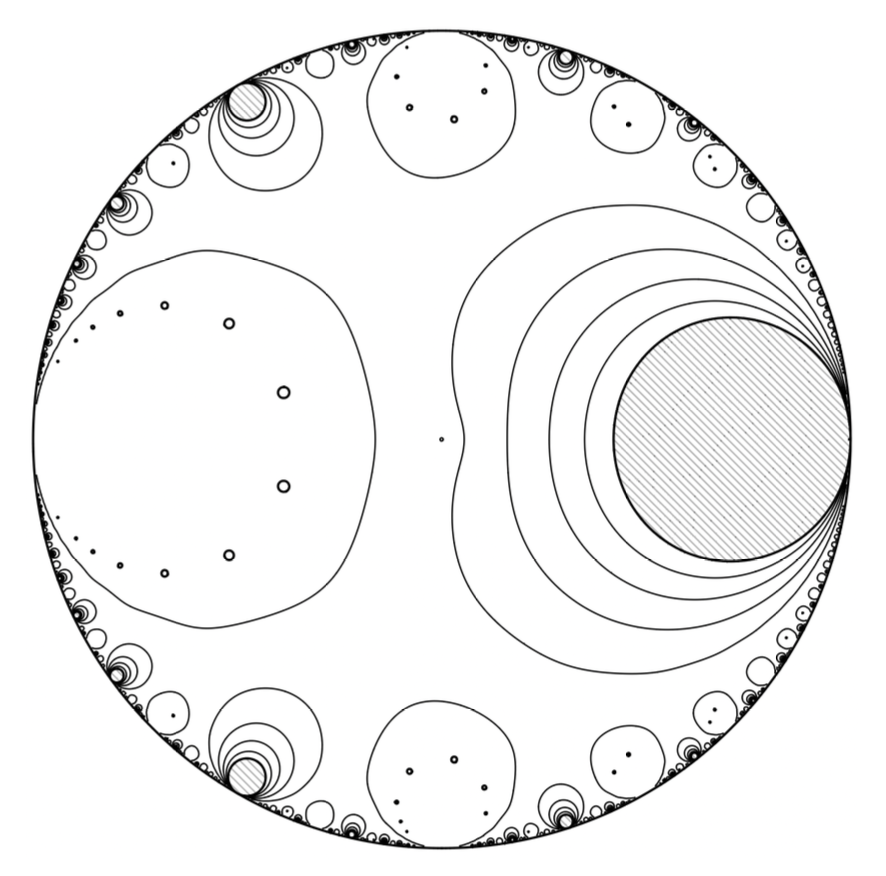
\includegraphics[width=0.45\textwidth]{src/psi1.png}%
        \label{fig:a}%
        }%
    \hfill%
    \subfloat{%
        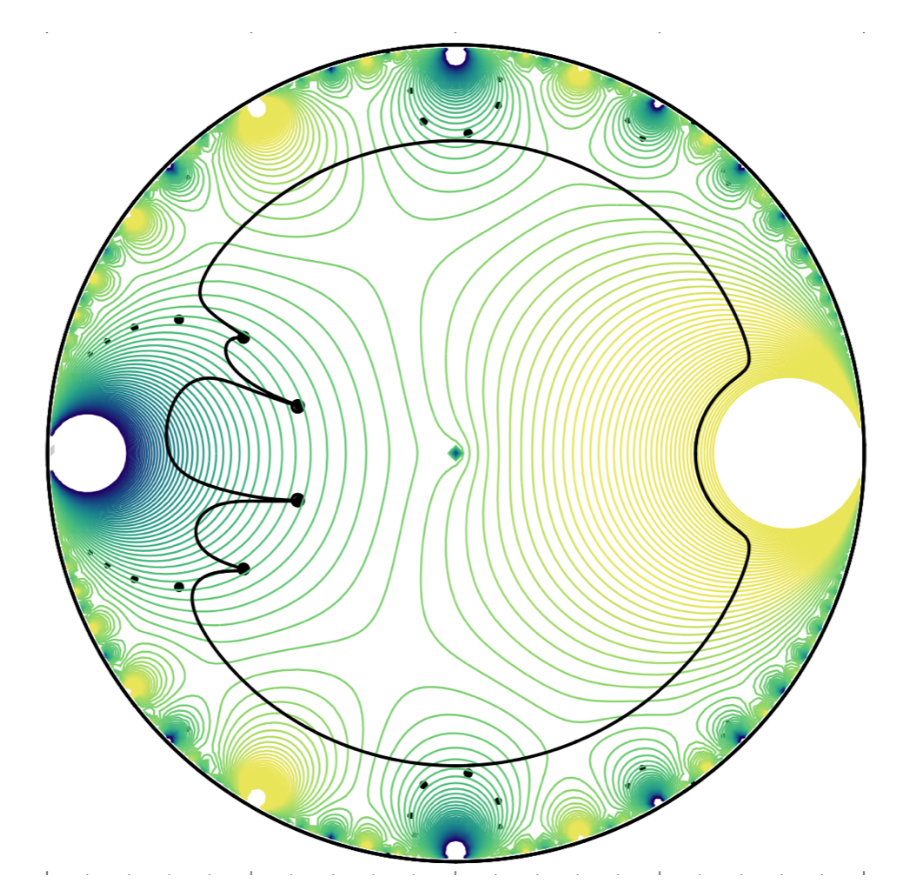
\includegraphics[width=0.47\textwidth]{src/psi2.png}%
        \label{fig:b}%
        }%
    \caption{Topography of $h$ (left, \cite[A.0.3]{calegari2024linear}) and the contour $\psi(\bT)$ (right, \cite[Figure A.4.5]{calegari2024linear})}
\end{figure}

\newpage
\section{Proof}

Now we are ready to prove the main result.

\begin{theorem}[{\cite[Theorem A]{calegari2024linear}}]
\label{thm:irrational}
$$
    L(2, \chi_{-3}) = \frac{1}{1^2} - \frac{1}{2^2} + \frac{1}{4^2} - \frac{1}{5^2} + \frac{1}{7^2} - \frac{1}{8^2} + \cdots
$$
is irrational. 
Moreover, $1, \zeta(2), L(2, \chi_{-3})$ are $\bQ$-linearly independent.
\end{theorem}

\begin{proof}
Assume $\bQ$-linear independence of $1, \zeta(2), L(2, \chi_{-3})$, so that there exist $a, b, c \in \bQ$ not all zero satisfying \eqref{eqn:lindep}.
As we mentioned before, this give 14 power series in $y$ that are $\bQ(y)$-linearly independent.
The denominator types of these series can be found in the below Table \ref{tab:denom} (we saw how the denominator types change under the symmetrization maps $\Sym^{\pm}$ from Daniel's talk - see \cite[Lemma 9.0.3]{calegari2024linear}).
The corresponding arrays $\mathbf{b}$ and $\mathbf{e}$ are
\begin{align*}
    \mathbf{b} &:= \begin{pmatrix}
        0 & 2 & 2 & 2 & 2 & 2 & 2 & 2 & 2 & 2 & 2 & 2 & 2 & 2 \\
        0 & 0 & 0 & 2 & 2 & 2 & 2 & 2 & 2 & 2 & 2 & 2 & 2 & 2
    \end{pmatrix}^\intercal \\
    \mathbf{e} &:= (0, 0, 1, 0, 0, 0, 0, 0, 0, 1, 1, 1, 1, 1).
\end{align*}
% \newpage

% \footnotesize
\begin{table}[t]
    \centering
    \begin{tabular}{ c|c } 
    function & denominator type \\
    \midrule
    \midrule
    $B_1$ & $1$ \\
     \midrule
    $B_2$ & $[1, \dots, 2n]$ \\
     \midrule
    $B_3$ & $n [1, \dots, 2n]$ \\
     \midrule
    $B_4$ & $[1, \dots, 2n]^2$\\
     \midrule
    $B_5$ & $(2n-1)[1, \dots, 2n]$\\
     \midrule
    $G$ & $[1, \dots, 2n]^2$ \\
     \midrule
    $G'$ & $[1, \dots, 2n+2]^2$ \\
     \midrule
    $G''$ & $[1, \dots, 2n+4]^2$ \\
     \midrule
    $G'''$ & $[1, \dots, 2n+6]^2$ \\
     \midrule
    $B_6$ & $n[1, \dots, 2n]^2$ \\
     \midrule
    $B_7$ & $n[1, \dots, 2n]^2$ \\
     \midrule
    $\int G(y) \dd y$ & $n[1, \dots, 2n-2]^2$ \\
     \midrule
    $\int \frac{G(y) - G(0)}{y} \dd y$ & $n[1, \dots, 2n]^2$ \\
     \midrule
    $\int \frac{G(y) - G(0) - G'(0)y}{y^2} \dd y$ & $n[1, \dots, 2n+2]^2$ \\
    \end{tabular}
    \caption{Denominator types}
    \label{tab:denom}
\end{table}


One can check analyticity (meromorphicity) of the pullbacks $\varphi^\ast F$ when $F$ is one of the series above, by applying Proposition \ref{prop:pullbackhol} with $\Sigma_{Y_0(2)}^0 = \{-\frac{1}{72}\}, \Sigma_{Y_0(2)}^1 = \emptyset, \varphi_{Y_0(2)} = \varphi$, and $U_{Y_0(2)}$ a sufficiently small open neighborhood of the line segment $[-\frac{1}{72}, 0]$, so we can apply Theorem \ref{thm:bound}.
(We also know that these have finite local monodromy of order dividing 2 at $y = 4$ by \cite[Lemma 9.0.3]{calegari2024linear}.)
We can compute $\tau(\mathbf{b}; \mathbf{e})$ explicitly, which is
$$
    \tau(\mathbf{b}; \mathbf{e}) = \tau^\flat(\mathbf{b}) + \tau^\sharp(\mathbf{e}) = \frac{191}{49} + \frac{27}{80} = \frac{16603}{3920} = 4.235459\dots.
$$
(For $\tau^\sharp(\mathbf{e})$, Figure \ref{fig:Igraph} shows the plot of the corresponding function $\xi \mapsto \frac{6\xi + I_{\xi}^{14}(\xi)}{98}$ which attains the minimum value of $\frac{27}{80}$ when $\xi \in [2, \frac{13}{6}]$).

\begin{figure}
    \centering
    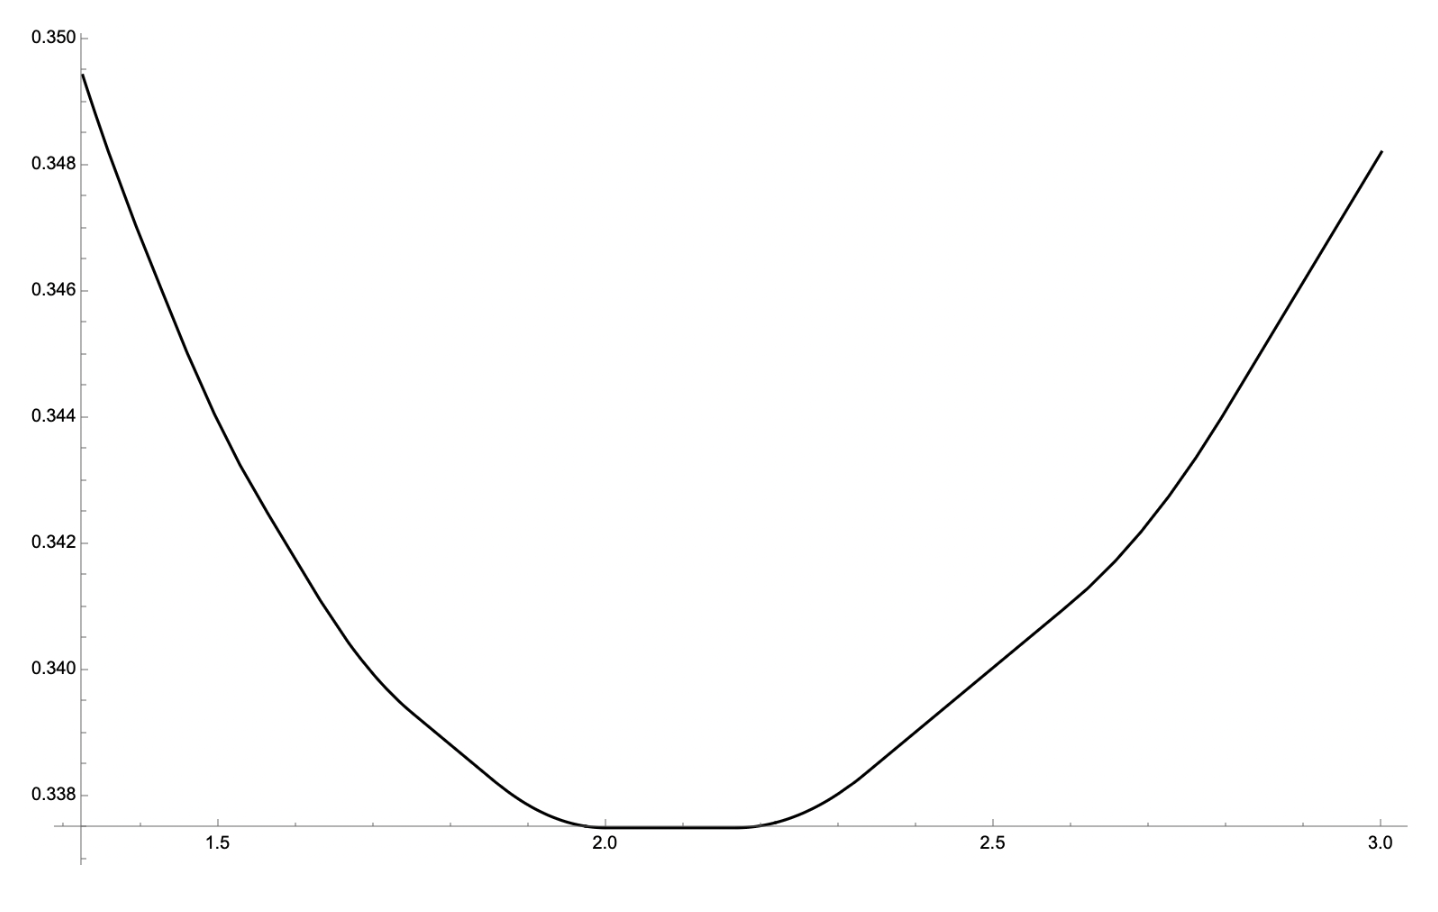
\includegraphics[width=0.8\linewidth]{src/Igraph.png}
    \caption{Plot of $\xi \mapsto \frac{6 \xi + I_{\xi}^{14}(\xi)}{98}$ on $[1.325, 3]$ \cite[Figure 13.0.3]{calegari2024linear}}
    \label{fig:Igraph}
\end{figure}

By definition of $\psi$ from Section \ref{sec:psi} (Equation \eqref{eqn:psi}), we have
$$
    |\varphi'(0)| = 256 \cdot c' \cdot R \cdot \frac{c^2 - 1}{c^2 + 1} \prod_{i=1}^{4} \frac{4r_i}{(1 + r_i)^{2}} = \frac{5448339453535586608000000000}{8658833407565631122430056127}.
$$
For the numerator, we can (numerically) compute the double integral with the explicit formula of $\varphi(z) = h(\psi(z))$, which gives
$$
    \iint_{\bT^2} \log |\varphi(z) - \varphi(w)| \dd \mu(z) \dd \mu(w) = 11.844\dots.
$$
Hence we get a holonomy bound
$$
    m \le \frac{11.845}{\log \left(\frac{5448339453535586608000000000}{8658833407565631122430056127}\right) - \frac{11603}{3920}} =13.9938 \dots < 14
$$
and get a contradiction.
\end{proof}

\begin{remark*}
You may found that the denominator types in Table \ref{tab:denom} are slightly larger than the numbers recorded in $\mathbf{b}$.
For example, $G'(y)$ has a denominator type of $[1, \dots, 2n + 2]^2$, not $[1, \dots, 2n]^2$.
This is not a problem, since one can replace it by $[1, \dots, (2 + \epsilon)n]^2$ for sufficiently small $\epsilon > 0$ for all but finitely many $n$'s, and the finite initial terms can be made to have any given denominator type by scaling, which yields the same bound as $\epsilon \to 0$ \cite[Remark 6.0.12]{calegari2024linear}.
\end{remark*}

\begin{remark*}
If we want to stick with a version of the theorem with $\mathbf{e} = \mathbf{0}$, one needs to append $\mathbf{e}$ to $\mathbf{b}$ (which is equivalent to replace $n^e$ with $[1, \dots, n]^e$ and get
\begin{align*}
    \mathbf{b}' := \begin{pmatrix}
        0 & 2 & 2 & 2 & 2 & 2 & 2 & 2 & 2 & 2 & 2 & 2 & 2 & 2 \\
        0 & 0 & 0 & 2 & 2 & 2 & 2 & 2 & 2 & 2 & 2 & 2 & 2 & 2 \\
        0 & 0 & 1 & 0 & 0 & 0 & 0 & 0 & 0 & 1 & 1 & 1 & 1 & 1
    \end{pmatrix}^\intercal 
\end{align*}
However, we cannot directly apply Theorem \ref{thm:bound} since the appended column is not in an increasing order.
In this case, one has a more general result \cite[Theorem 8.0.1]{calegari2024linear} allowing such relaxations at the cost of a worse bound.
We need to replace $\tau^\flat(\mathbf{b}) + \tau^\sharp(\mathbf{e})$ with $\tau^{\flat\flat}(\mathbf{b}')$ (where the definition can be found in \cite[Equation 8.0.2]{calegari2024linear}), which is at least
$$
    \tau^{\flat\flat}(\mathbf{b}') \ge \frac{884}{196} = 4.510\dots,
$$
significantly worse than the above $\tau(\mathbf{b};\mathbf{e}) = 4.2354\dots$ and not enough to get a dimension bound less than 14.
\end{remark*}

\begin{remark*}
One may not happy about the possible numerical issue when we compute the double integral.
The authors used \texttt{mathematica} to estimate the integral, and the formula of $h(q)$ and $\psi(x)$ are explicit enough to estimate the integral as accurately as we want.
Alternatively, there are two other holonomy bounds (Theorem 6.0.2 and Theorem 7.1.6 of \cite{calegari2024linear}) which are much more complicated but gives a better numerical stability, and strong enough to yield similar contradictions.
\end{remark*}
\section{Product of two logarithms}

In \cite{calegari2024linear}, the authors also proved irrationality result for the product of log values.
More precisely, they proved the following theorem:
\begin{theorem}[{\cite[Theorem 14.0.1]{calegari2024linear}}]
Let $m, n \in \bZ \backslash \{-1, 0\}$ be integers such that $\left|\frac{n}{m} - 1\right| < 10^{-6}$.
Then
$$
    \log \left(1 + \frac{1}{m}\right) \log \left(1 + \frac{1}{n}\right)
$$
is irrational.
Moreover, for $m \ne n$, the following are linearly independent over $\bQ$:
\begin{equation}
\label{eqn:log}
    1, \quad \log \left(1 + \frac{1}{m}\right), \quad \log \left(1 + \frac{1}{n} \right), \quad \log \left(1 + \frac{1}{m}\right) \log \left(1 + \frac{1}{n}\right).
\end{equation}
\end{theorem}
Proof uses the same idea (holonomy bound) with different series.
More precisely, let $a = 2m + 1, b = 2n+1$ and define
\begin{align*}
    A(a, x) &:= \frac{1}{\sqrt{1 - 2ax + x^2}} \\
    H(a, x) &:= \frac{1}{\sqrt{1 - 2ax + x^2}} \int_{0}^{x} \frac{\dd t}{\sqrt{1 - 2at + t^2}}
\end{align*}
where both lies in $\bQ \llb x \rrb$ and satisfy first order ODEs.
These have singularities at $a \pm \sqrt{a^2 - 1}$.
Assume that there exist integers $r_0, r_a, r_b, r_{ab}$ not all zero such that
$$
    r_a \cdot \frac{1}{2} \log \left(\frac{a + 1}{a - 1}\right) + r_b \cdot \frac{1}{2} \log \left(\frac{b + 1}{b - 1}\right) + r_{ab} \cdot \frac{1}{4} \log \left(\frac{a + 1}{a - 1}\right) \log \left(\frac{b + 1}{b - 1}\right) = r_0.
$$
We use the same 7 functions $B_1, \dots, B_7$ along with new (hypothetical) 10 functions coming from differentiations and integrals of a (hypothetical) $G$-function $G(y) = \Sym^+ P(x) \in \bQ \llb y \rrb$ where
\begin{align*}
    P(x) &= r_a P_a + r_b P_b + r_{ab} P_{ab} \\
    P_a(x) &= \left(H(a, x) - \frac{1}{2} \log \left(\frac{a+1}{a-1}\right) \right) \,\star A(b, x)  \\
    P_b(x) &= \left(H(b, x) - \frac{1}{2} \log \left(\frac{b+1}{b-1}\right)\right) \,\star A(a, x)  \\
    P_{ab}(x) &= H(a, x) \,\star H(b, x) - \frac{1}{4} \log \left(\frac{a+1}{a-1} \right) \log \left(\frac{b+1}{b-1}\right) A(a, x) \,\star A(b, x)
\end{align*}
where $\star$ is the Hadamard product (coefficient-wise product of two power series).
Now, the following 17 functions
\begin{align*}
    &B_1(y), \quad B_2(y), \quad B_3(y), \quad B_4(y), \quad B_5(y), \\
    &G(y), \quad G'(y), \quad G''(y), \quad G'''(y), \\
    &B_6(y), \quad B_7(y), \quad \int y G(y) \dd y, \quad \int G(y) \dd y, \quad \int \frac{G(y) - G(0)}{y} \dd y, \\
    &\int \frac{G(y) - G(0) - G'(0)y}{y^2} \dd y, \quad \int \frac{G(y) - G(0) - G'(0)y - G''(0) \frac{y^2}{2}}{y^3} \dd y,\\
    &\int \frac{G(y) - G(0) - G'(0)y - G''(0) \frac{y^2}{2} - G'''(y) \frac{y^3}{6}}{y^4} \dd y
\end{align*}
are $\bQ(y)$-linearly independent (in fact, $\bC(y)$-linearly independent), and have denominator types of $n [1, \dots, 2n]^2$.
More precisely, the corresponding array $\mathbf{b}$ and $\mathbf{e}$ are
\begin{align*}
    \mathbf{b} &:= \begin{pmatrix}
        0 & 2 & 2 & 2 & 2 & 2 & 2 & 2 & 2 & 2 & 2 & 2 & 2 & 2 & 2 & 2 & 2 \\
        0 & 0 & 0 & 2 & 2 & 2 & 2 & 2 & 2 & 2 & 2 & 2 & 2 & 2 & 2 & 2 & 2
    \end{pmatrix}^\intercal \\
    \mathbf{e} &:= (0, 0, 1, 0, 0, 0, 0, 0, 0, 1, 1, 1, 1, 1, 1, 1, 1).
\end{align*}
Using Proposition \ref{prop:pullbackhol} again with $\Sigma_{Y_0(2)}^0 = \{y_{a^-, b^-}\}$, $\Sigma_{Y_0(2)}^1 = \emptyset$, and $U_{Y_0(2)} = D(0, \frac{1}{100})$, where $y_{a^-, b^-}$ is the image of $(a - \sqrt{a^2 - 1})(b - \sqrt{b^2 - 1})$ under the symmetrizing map $x \mapsto y(x)$, one can check holomorphicity of the pullbacks of 17 functions under the same $\varphi$ we used for Theorem \ref{thm:irrational}.
Now explicit computation gives
$$
    \tau(\mathbf{b}; \mathbf{e}) = \frac{1136}{289} + \frac{78419}{242760} = \frac{1032659}{242760} = 4.2538\dots
$$
and the corresponding holonomy bound is around $16.2 < 17$, which gives a contradiction and proves linear independence of the four numbers in \eqref{eqn:log}.

In the proof, we use the assumption that $\frac{a}{b}$ is close to $1$, to ensure that 1) the singularities of $P_a(x)$ and $P_b(x)$ are close to $0$ and $\infty$, and 2) the singularities of $P_{ab}(x)$ are close to $0$, $1$, and $\infty$.
The assumption is also used in the proof of linear independence, although we need a weaker assumption for the purpose.
\newpage


% --- Bibliography ---

% Start a bibliography with one item.
% Citation example: "\cite{williams}".

\bibliographystyle{acm} % We choose the "plain" reference style
\bibliography{refs} % Entries are in the refs.bib file


% \begin{thebibliography}{1}

% \bibitem{williams}
%    Williams, David.
%    \textit{Probability with Martingales}.
%    Cambridge University Press, 1991.
%    Print.

% % Uncomment the following lines to include a webpage
% % \bibitem{webpage1}
% %   LastName, FirstName. ``Webpage Title''.
% %   WebsiteName, OrganizationName.
% %   Online; accessed Month Date, Year.\\
% %   \texttt{www.URLhere.com}

% \end{thebibliography}

% --- Document ends here ---

\end{document}